\section{Proposed Solution}

This proposed solution as an improved user interaction concept allows for a very
flexible and interactive \gls{pims} allowing the user
The proposal: An atomic data management system utilizing a smartwatch to take advantage of faster and more instantaneous data input.
The here proposed solution features a \gls{pims} supporting relationships
between bits of information. Since the proposed solution does not store
information sequentially but relationally, the reorganization of existing
information is possible without changing the information itself.

% deals with chunks of data

\subsection{Unstructured Data}

Various types of unstructured data can be seen in figure \ref{fig:unstructdata}
but unstructured data doesn't oppose any restrictions upon the user of the
\gls{pims} or what the implementation of such system itself. Basic
implementations can stick to text and graphical data. However, as the system
grows so do the needs of the user.

\begin{flfigure}
  \centering
    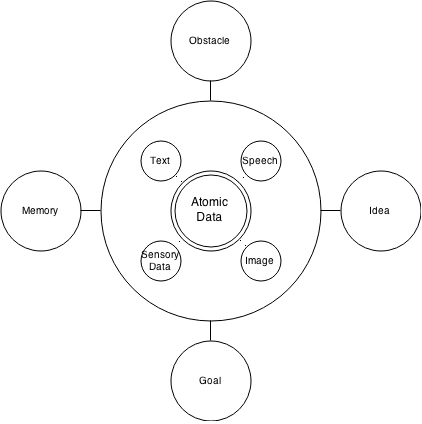
\includegraphics[width=0.9\linewidth]{00_resources/atomic_data.png}
    \caption{Unstructured data}
  \label{fig:unstructdata}
\end{flfigure}

Chunks of unstructured data can then be connected to other chunks by the user of
the system. The finer the chunks are, the more flexibility does the user have in
creating connections between chunks. A letter, for instance, can be inserted
into the system as one chunk of data which does not allow any connections within
the letter itself. However, the letter could also be inserted as multiple chunks
allowing the user to connect pieces of the letter to itself or other
information within the \gls{pims}.

\subsection{Data Sources}

In principle, any platform that implements a \gls{pims} that adheres to this
proposal can be a data source. However, this system is not meant to be
restricted to a particular platform but more so be a hub where any platform the
user chooses is supported in such a way that data can be inserted by the user.
Figure \ref{fig:datasources} shows a diagram of possible data sources across
multiple platforms.

\begin{flfigure}
  \centering
    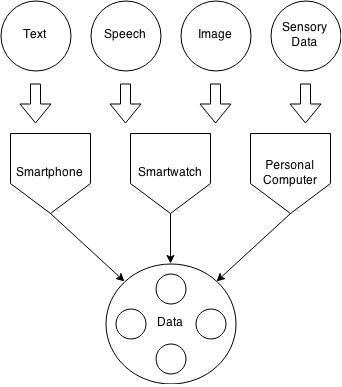
\includegraphics[width=0.9\linewidth]{00_resources/input_methods.png}
    \caption{Variety of data sources}
  \label{fig:datasources}
\end{flfigure}

\subsection{Organization of Data}

The organization of unstructured data is on a par with the available
visualizations thereof. That means that a \gls{pims} implementing all presented
visualizations allows the organization of unstructured data by any of those
visualizations or a combination thereof.

For instance, a system that supports connections between unstructured data and
a coordinate system must allow the user to connect chunks of unstructured data
with each other and simultaneously place these same chunks on a coordinate system.
A system need not support all visualizations presented in this paper or can
implement further visualizations not presented here.

Previously inserted atomic bits of data can be organized using a variety of models which are not all specified in this document. The more obvious ones are folders and labels as well as relationships between atomic data which can then be visualized as maps and radial relationship diagrams.

\subsection{Connections of Data}

Chunks of unstructured data can be connected to other chunks as shown in figure
\ref{fig:visualconnections}. The visualization can resemble a two-dimensional
map showing all chunks of data including its connections or can lean toward a
radial graph where the user can move through the connections by changing the
chunk in the center.

\begin{flfigure}
  \centering
    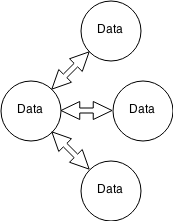
\includegraphics[width=0.5\linewidth]{00_resources/data_connections.png}
    \caption{Visualized relationships of unstructured data}
  \label{fig:visualconnections}
\end{flfigure}

\subsubsection{Labels}

Figure \ref{fig:visuallabels} shows the organization of chunks of data by
folders, here called labels. The visual representation looks quite similar to
the figure but can take other forms.

\begin{flfigure}
  \centering
    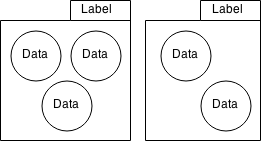
\includegraphics[width=0.5\linewidth]{00_resources/data_labels.png}
    \caption{Visualized labels of unstructured data}
  \label{fig:visuallabels}
\end{flfigure}

\subsubsection{Timeline}

\begin{flfigure}
  \centering
    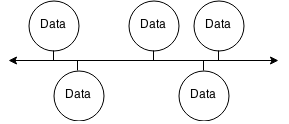
\includegraphics[width=0.5\linewidth]{00_resources/data_timeline.png}
    \caption{Visual timeline of unstructured data}
  \label{fig:visualtimeline}
\end{flfigure}

Data atoms can be ordered by time either manually specified or by the creation time of the data atom itself.

\subsubsection{Matrix}

\begin{flfigure}
  \centering
    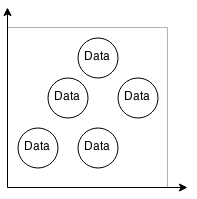
\includegraphics[width=0.5\linewidth]{00_resources/data_coord_system.png}
    \caption{Visual two-dimensional coordinate system of unstructured data}
  \label{fig:visualcoordsys}
\end{flfigure}

As seen in figure \ref{fig:visualcoordsys}, ...
Data atoms can be part of a two-dimensional matrix which can then be visualized.
